\section{Chasis del módulo interior}
\label{app:diseno-interior}

\subsection{Lista de materiales}

\vfill

\begin{table}[H]
\caption{Lista de materiales del módulo interior (chasis)}
\label{tab:materiales-carcasa-interior}
\begin{tabularx}{\textwidth}{cX}
\toprule
\headingc{Cantidad} & \headingc{Descripción} \\
\topruleb
1 & Hoja de metacrilato de 3mm de grosor (270mm x 90mm)\\*\midrule
8 & Tuercas de nylon M3 nylon hex nuts\\*\midrule
8 & Tornillos de nylon con cabeza Phillips M3 x 6mm\\*\midrule
4 & Tornillo de nylon con tuerca integrada M3 x 6mm + 6mm\\*\bottomrule
\end{tabularx}
\end{table}

\vfill

\subsection{Boceto del chasis del módulo interior}

\vfill

\begin{figure}[H]
  \centering
  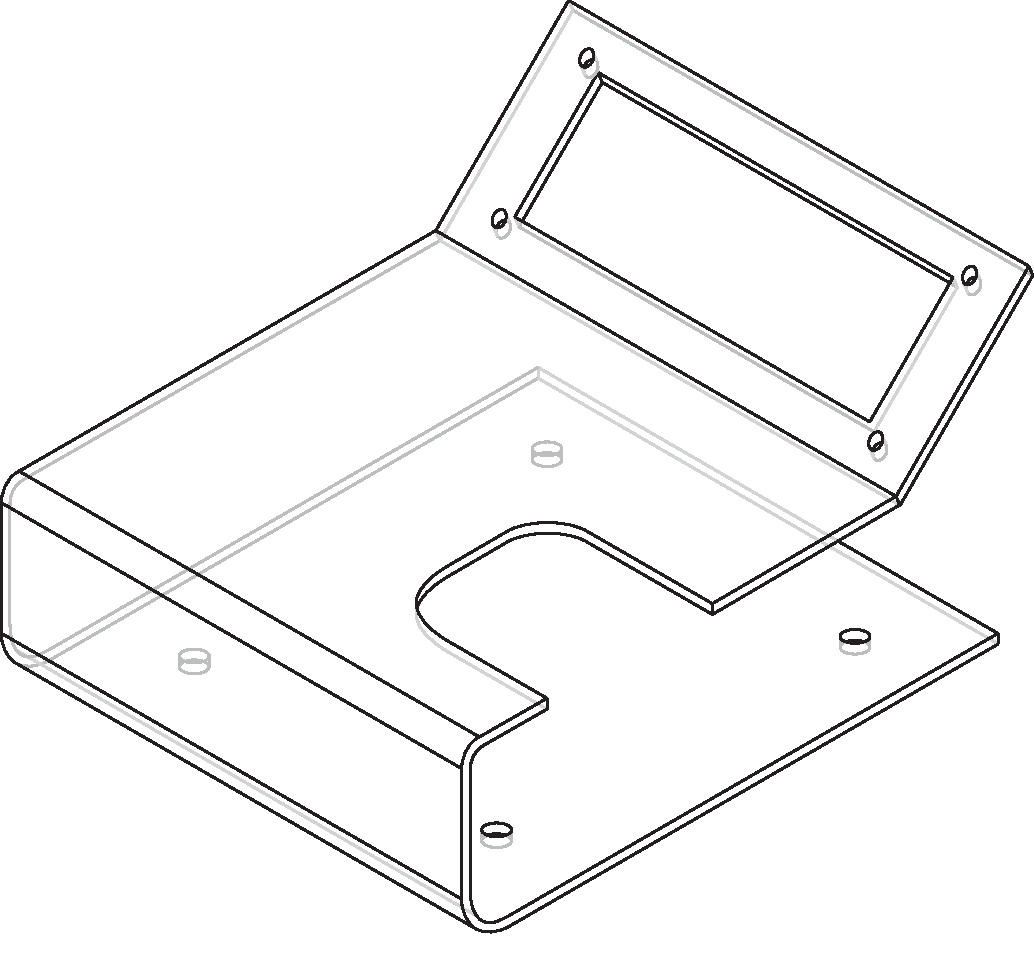
\includegraphics[width=0.53\columnwidth]{../design/interior-body-design}
  \caption{Boceto del chasis del módulo interior}
  \label{fig:interior-body-design}
\end{figure}

\vfill

\clearpage

\subsection{Mecanizado del chasis del módulo interior}

\vfill

\begin{figure}[H]
  \centering
  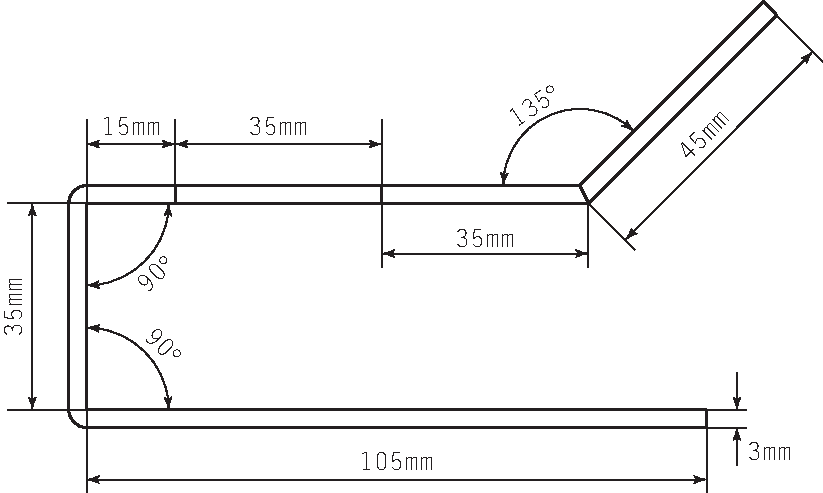
\includegraphics[width=0.8\columnwidth]{../design/interior-body-side}
  \caption{Doblado del chasis del módulo interior (vista lateral)}
  \label{fig:interior-body-side}
\end{figure}

\vfill

\clearpage

\begin{figure}
  \centering
  \includegraphics[height=0.98\textheight]{../design/interior-body-blueprint}
  \caption{Diseño del corte del chasis del módulo interior}
  \label{fig:interior-body-blueprint}
\end{figure}


